\documentclass[../lecture2-variablesandcontrolstructures.tex]{subfiles}

\begin{document}

\section{Misc}

% -------------------------------------------------------------------

\begin{frame}[fragile]{Initialization of Variables}
t
\end{frame}

% -------------------------------------------------------------------

\begin{frame}[fragile]{Expressions with Mixed Variable Types (Type Casting)}
sometimes you want to change somthings type, this is called typecasting

(float)5 = 5.0
(int)5.0 = 5

note when converting to a less precise type information is lost
e.g. (int)5.1 = 5
     (int)5.9 = 5

\end{frame}

% -------------------------------------------------------------------

\begin{frame}[fragile]{Declaration and Initialization of Symbolic Constants}
#define MY_NUMBER 5

in the code MY_NUMBER will now be replaced with 5
\end{frame}

% -------------------------------------------------------------------

\begin{frame}[fragile]{Check this out}
    \begin{center}
        \makebox[\textwidth]{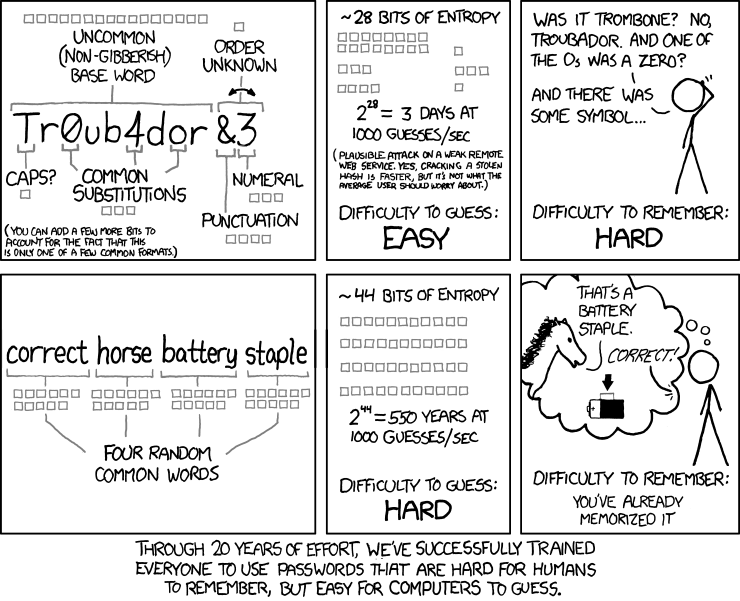
\includegraphics[width=0.95\paperwidth,height=0.85\paperheight]{graphics/xkcd-password_strength.png}}
    \end{center}
\end{frame}

% -------------------------------------------------------------------

\end{document}
